\documentclass[12pt,a4paper]{article}

% ---------------- Налаштування ----------------
\usepackage{fontspec}   % кодуваніня
\setmainfont{Times New Roman}
\setmonofont{Courier New}
\usepackage[ukrainian]{babel} % українська мова
\usepackage{amsmath, amssymb} % математика
\usepackage{graphicx}         % вставка картинок
\usepackage{hyperref}         % клікабельні посилання
\usepackage{geometry}         % поля
\usepackage{float}
\usepackage{booktabs} % Для красивых линий
\usepackage{caption}  % Для подписей

\geometry{left=25mm,right=15mm,top=20mm,bottom=20mm}

\usepackage{listings}
\lstset{
    basicstyle=\ttfamily,
    inputencoding=utf8,   
    extendedchars=true,    
    breaklines=true
}

\usepackage{fancyhdr}
\setlength{\headheight}{14.5pt} % мінімум для fancyhdr
\pagestyle{fancy}
\fancyhf{}
\lhead{Протокол лабораторної роботи}
\rhead{\thepage}

\lstset{
    basicstyle=\ttfamily,
    inputencoding=utf8,
    extendedchars=true,
    breaklines=true,
    columns=fullflexible
}

% ---------------- Титул ----------------
\begin{document}

\begin{titlepage}
\centering
Міністерство освіти і науки України \\
НТУУ «Київський політехнічний інститут» \\
Фізико-технічний інститут
\vfill

\textbf{Протокол лабораторної роботи №1} \\ % номер лабораторної роботи
з дисципліни Проектування високонавантажених систем \\ % назва курсу
на тему: Порівняння пропускної здатності
\vfill

\begin{flushright}
Виконав: студент групи ФІ-21 \\
Грунда Ярослав \\
\end{flushright}

\vfill
Київ, 2025
\end{titlepage}

% ---------------- Основна частина ----------------
\section*{Мета роботи}
Порівняти throughput (пропускна здатність) Веб-застосунку в залежності від навантаження та способу зберігання даних (в памʼяті та БД).


\section*{Завдання}
\begin{enumerate}
\item Створити Веб-застосунок який містить два ендпоінта (приймає два запити):\\
\begin{itemize}
\item /inc - інкрементує внутрішній каунтер\\
\item /count - повертає значення каунтера\\
\end{itemize}
\item Cтворити HTTP-клієнта, який зможе робити задану кількість викликів до Веб-застосунку, а також заміряти час витрачений на здійснення цих викликів.
\item Порівняти пропускну здатність в залежності від кількості клієнтів (1, 2, 5, 10) та способу зберігання даних (в памʼяті та БД). 
Кожен клієнт робить по 10 тисяч викликів.
\item Веб-застосунок має підтримувати багатопоточність.
\item Клієнти мають запускатись паралельно та одночасно генерувати запити.
\item Каунтер на Веб-застосунку має бути потоко-безпечним та забезпечувати відсутність lost-update.
\end{enumerate}
\tableofcontents
\newpage
\section{Результати}
\begin{table}[h!]
  \centering
  \caption{In-memory testing}
  \label{tab:in_memory_testing}
  \begin{tabular}{lcccc}
    \toprule
    \textbf{Number of clients} & \textbf{Expected count} & \textbf{Actual count} & \textbf{Total time (s)} & \textbf{Throughput (req/s)} \\
    \midrule
    1 & 10,000 & 10,000 & 8.7780 & 1,139.21 \\
    2 & 20,000 & 20,000 & 13.8720 & 1,441.75 \\
    5 & 50,000 & 50,000 & 37.0491 & 1,349.56 \\
    10 & 100,000 & 100,000 & 75.0806 & 1,331.90 \\
    \bottomrule
  \end{tabular}
\end{table}
\begin{table}[h!]
  \centering
  \caption{DB testing}
  \label{tab:db_testing}
  \begin{tabular}{lcccc}
    \toprule
    \textbf{Number of clients} & \textbf{Expected count} & \textbf{Actual count} & \textbf{Total time (s)} & \textbf{Throughput (req/s)} \\
    \midrule
    1 & 10,000 & 10,000 & 14.0577 & 711.35 \\
    2 & 20,000 & 20,000 & 16.5079 & 1,211.54 \\
    5 & 50,000 & 50,000 & 42.2388 & 1,183.74 \\
    10 & 100,000 & 100,000 & 82.1198 & 1,217.73 \\
    \bottomrule
  \end{tabular}
\end{table}

\newpage
\section{Скриншоти результатів}
\begin{figure}[h!]
  \centering
  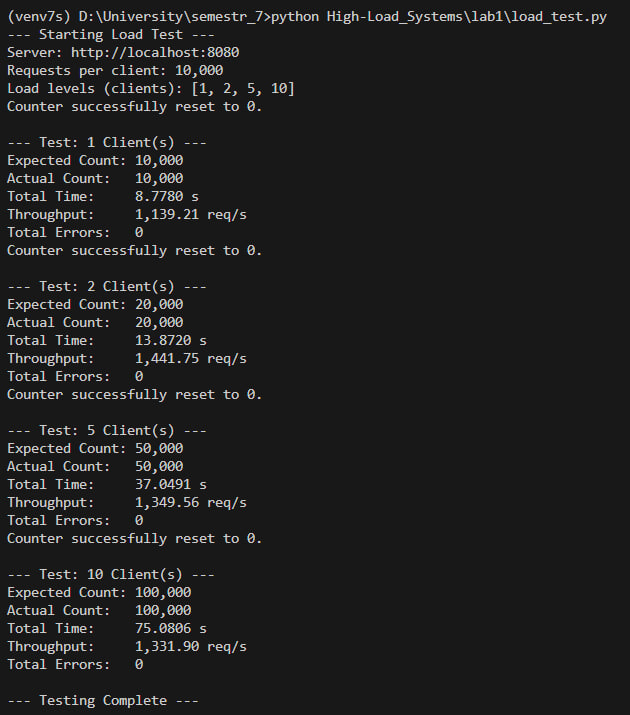
\includegraphics[scale=0.5]{../imgs/in_memory.jpg}
  \caption{In-memory testing}
  \label{fig:in_memory}
\end{figure}
\begin{figure}[h!]
  \centering
  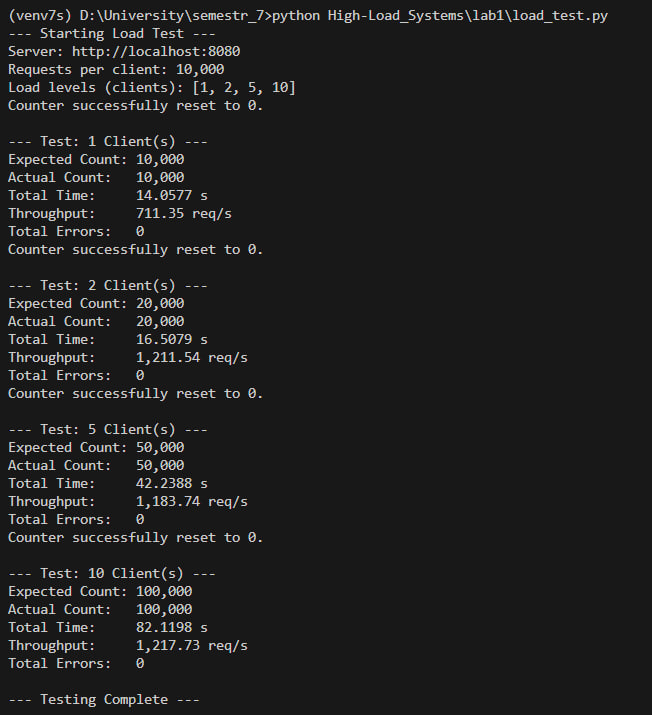
\includegraphics[scale=0.5]{../imgs/db.jpg}
  \caption{DB testing}
  \label{fig:db}
\end{figure}

\section{Висновки}
\subsection{Порівняння Пропускної Здатності}

\textbf{In-Memory Server (зберігання в пам'яті)}\\
При 1 клієнті цей сервер показав високу базову пропускну здатність (~1139 req/s), 
а пікове значення продуктивності було досягнуто при 2 клієнтах (~1441 req/s).
При 5 та 10 клієнтах пропускна здатність почала незначно знижуватися (~1349 та ~1331 req/s відповідно). 
Це пояснюється зростанням конкуренції (contention) за доступ до єдиної атомарної змінної, що створює невеликі затримки.\\
\textbf{DB Server (зберігання в базі даних)}\\
При 1 клієнті сервер продемонстрував найнижчу пропускну здатність (~711 req/s) через накладні витрати на мережеву взаємодію з БД.
З ростом кількості клієнтів продуктивність значно зростала і стабілізувалася на високому рівні (~1211-1217 req/s). 
Це демонструє здатність PostgreSQL ефективно обробляти паралельні запити, використовуючи пул з'єднань та внутрішні механізми паралелізму.\\
\textbf{Загальний висновок}\\
In-Memory рішення є беззаперечним лідером за швидкістю, проте дані при цьому є тимчасовими. 
На противагу, сервер з базою даних надає найважливішу перевагу — персистентність (надійне збереження стану), 
а також краще масштабується під високим навантаженням, що робить його більш стійким та практичним рішенням.
\subsection{Реалізація Технічних Вимог}
\begin{enumerate}
\item Багатопоточність веб-застосунку: Обидва веб-сервери, написані на Go, за замовчуванням є багатопоточними. Стандартний пакет net/http автоматично обробляє кожен вхідний HTTP-запит у власній горутині (goroutine), що забезпечує високий рівень паралелізму без додаткового коду.
\item Паралельний запуск клієнтів: У Python-скрипті load\_test.py для одночасного генерування запитів було використано бібліотеку concurrent.futures та клас ThreadPoolExecutor.
\item Потокобезпечний каунтер: Проблема lost updates була вирішена двома різними методами:
\begin{itemize}
\item Для in\_memory\_server використовувався пакет sync/atomic та тип atomic.Int64. Його метод Add(1) виконує операцію інкременту на апаратному рівні як єдину неподільну (атомарну) інструкцію, що унеможливлює виникнення гонки даних.
\item Для db\_server потоко-безпечність забезпечувалася самою системою управління базами даних PostgreSQL.
\end{itemize}
\end{enumerate}

\section{Код}
Посилання на репозиторій: \href{https://github.com/gre1wy/High-Load_Systems/tree/main/lab1}{GitHub}
\subsection{Clients}
\begin{verbatim}
# File: load_test.py
import requests
import time
import argparse
from concurrent.futures import ThreadPoolExecutor, as_completed

# --- Configuration ---
DEFAULT_BASE_URL = "http://localhost:8080"
DEFAULT_REQUESTS_PER_CLIENT = 10000
DEFAULT_CLIENT_LOADS = [1, 2, 5, 10]

def reset_counter(base_url):
    """Sends a request to /reset to reset the counter on the server."""
    try:
        response = requests.get(f"{base_url}/reset", timeout=5)
        response.raise_for_status()
        print("Counter successfully reset to 0.")
        return True
    except requests.RequestException as e:
        print(f"Failed to reset counter: {e}")
        return False

def make_requests(client_id, base_url, requests_per_client):
    """
    Thread function: performs a given number of /inc requests.
    Returns the number of errors that occurred during execution.
    """
    error_count = 0
    with requests.Session() as session:
        for _ in range(requests_per_client):
            try:
                # Set a short timeout to avoid waiting forever
                response = session.get(f"{base_url}/inc", timeout=2)
                response.raise_for_status()
            except requests.RequestException:
                error_count += 1
    return error_count

def get_final_count(base_url):
    """Gets the final value of /count"""
    try:
        response = requests.get(f"{base_url}/count", timeout=5)
        response.raise_for_status()
        return int(response.text.strip())
    except (requests.RequestException, ValueError) as e:
        print(f"Failed to get the final count: {e}")
        return "ERROR"

def run_test(num_clients, base_url, requests_per_client):
    """Runs a load test with N clients"""
    print(f"\n--- Test: {num_clients} Client(s) ---")
    
    start_time = time.time()
    total_errors = 0
    
    with ThreadPoolExecutor(max_workers=num_clients) as executor:
        # Create tasks for each client
        futures = [executor.submit(make_requests, i, base_url, 
            requests_per_client) for i in range(num_clients)]
        
        # Collect results as they complete
        for future in as_completed(futures):
            total_errors += future.result()

    end_time = time.time()
    total_time = end_time - start_time
    total_requests = num_clients * requests_per_client
    
    throughput = total_requests / total_time
    final_count = get_final_count(base_url)
    
    print(f"Expected Count: {total_requests:,}")
    print(f"Actual Count:   {final_count:,}" if isinstance(final_count, int) else f"Actual Count:   {final_count}")
    print(f"Total Time:     {total_time:.4f} s")
    print(f"Throughput:     {throughput:,.2f} req/s")
    print(f"Total Errors:   {total_errors:,}")
    
    # Correctness check
    if isinstance(final_count, int) and final_count != total_requests:
         print("WARNING: Actual and expected counts do not match! Possible race condition on the server.")

if __name__ == "__main__":
    parser = argparse.ArgumentParser(description="A script for load testing a web counter.")
    parser.add_argument("--url", default=DEFAULT_BASE_URL, help="Server URL, e.g., http://localhost:8080")
    parser.add_argument("--reqs", type=int, default=DEFAULT_REQUESTS_PER_CLIENT, help="Number of requests per client")
    parser.add_argument("--clients", nargs='+', type=int, default=DEFAULT_CLIENT_LOADS, help="List of client loads, e.g., 1 5 10")
    args = parser.parse_args()

    print("--- Starting Load Test ---")
    print(f"Server: {args.url}")
    print(f"Requests per client: {args.reqs:,}")
    print(f"Load levels (clients): {args.clients}")

    for client_count in args.clients:
        # 1. Reset the counter before each test
        if not reset_counter(args.url):
            break # Abort if reset fails

        # 2. Brief pause to ensure the server is ready
        time.sleep(1)

        # 3. Run the test
        run_test(client_count, args.url, args.reqs)

    print("\n--- Testing Complete ---")
\end{verbatim}
\subsection{In-memory Server}
\begin{verbatim}
    // File: in_memory_server.go
package main

import (
	"context"
	"fmt"
	"log/slog"
	"net/http"
	"os"
	"os/signal"
	"sync/atomic"
	"syscall"
	"time"
)

// WebCounter uses atomic.Int64 for maximum performance.
type WebCounter struct {
	count atomic.Int64
}

// IncHandler atomically increments the counter by 1.
func (wc *WebCounter) IncHandler(w http.ResponseWriter, r *http.Request) {
	wc.count.Add(1)
	w.WriteHeader(http.StatusOK)
}

// CountHandler atomically reads the current value of the counter.
func (wc *WebCounter) CountHandler(w http.ResponseWriter, r *http.Request) {
	currentCount := wc.count.Load()
	w.Header().Set("Content-Type", "text/plain")
	fmt.Fprintf(w, "%d", currentCount)
}

// ResetHandler atomically resets the counter to 0.
func (wc *WebCounter) ResetHandler(w http.ResponseWriter, r *http.Request) {
	wc.count.Store(0)
	w.Header().Set("Content-Type", "text/plain")
	fmt.Fprintln(w, "Counter reset to 0")
}

func main() {
	logger := slog.New(slog.NewJSONHandler(os.Stdout, nil))
	slog.SetDefault(logger)

	counter := &WebCounter{}

	mux := http.NewServeMux()
	mux.HandleFunc("/inc", counter.IncHandler)
	mux.HandleFunc("/count", counter.CountHandler)
	mux.HandleFunc("/reset", counter.ResetHandler)

	server := &http.Server{
		Addr:    ":8080",
		Handler: mux,
	}

	// Start the server in a separate goroutine
	go func() {
		slog.Info("Starting In-Memory server on", "addr", server.Addr)
		if err := server.ListenAndServe(); err != nil && err != http.ErrServerClosed {
			slog.Error("Server failed to start", "error", err)
			os.Exit(1)
		}
	}()

	// Graceful Shutdown implementation
	stopChan := make(chan os.Signal, 1)
	signal.Notify(stopChan, syscall.SIGINT, syscall.SIGTERM) // Catch Ctrl+C and kill signals

	<-stopChan // Block until a signal is received

	slog.Info("Shutting down server gracefully...")

	// Allow 5 seconds for current requests to finish
	ctx, cancel := context.WithTimeout(context.Background(), 5*time.Second)
	defer cancel()

	if err := server.Shutdown(ctx); err != nil {
		slog.Error("Graceful shutdown failed", "error", err)
	} else {
		slog.Info("Server stopped gracefully")
	}
}

\end{verbatim}
\subsection{DB Server}
\begin{verbatim}
    // File: db_server.go
package main

import (
	"context"
	"database/sql"
	"fmt"
	"log/slog"
	"net/http"
	"os"
	"os/signal"
	"syscall"
	"time"

	_ "github.com/lib/pq"
)

// DBWrapper contains the database connection.
type DBWrapper struct {
	DB *sql.DB
}

// IncHandler uses ExecContext for a thread-safe increment in the DB.
func (dw *DBWrapper) IncHandler(w http.ResponseWriter, r *http.Request) {
	_, err := dw.DB.ExecContext(r.Context(), "UPDATE counter_table SET value = value + 1 WHERE id = 1")
	if err != nil {
		slog.Error("DB error during increment", "error", err)
		http.Error(w, "DB error", http.StatusInternalServerError)
		return
	}
	w.WriteHeader(http.StatusOK)
}

// CountHandler uses QueryRowContext to read the value.
func (dw *DBWrapper) CountHandler(w http.ResponseWriter, r *http.Request) {
	var count int64
	err := dw.DB.QueryRowContext(r.Context(), "SELECT value FROM counter_table WHERE id = 1").Scan(&count)
	if err != nil {
		slog.Error("DB error during read", "error", err)
		http.Error(w, "DB error", http.StatusInternalServerError)
		return
	}
	w.Header().Set("Content-Type", "text/plain")
	fmt.Fprintf(w, "%d", count)
}

// ResetHandler resets the counter in the DB.
func (dw *DBWrapper) ResetHandler(w http.ResponseWriter, r *http.Request) {
	_, err := dw.DB.ExecContext(r.Context(), "UPDATE counter_table SET value = 0 WHERE id = 1")
	if err != nil {
		slog.Error("DB error during reset", "error", err)
		http.Error(w, "DB error", http.StatusInternalServerError)
		return
	}
	w.Header().Set("Content-Type", "text/plain")
	fmt.Fprintln(w, "Counter reset to 0 in DB")
}

func main() {
	logger := slog.New(slog.NewJSONHandler(os.Stdout, nil))
	slog.SetDefault(logger)

	// --- Get the connection string from an environment variable ---
	connStr := os.Getenv("DATABASE_URL")
	if connStr == "" {
		// Default value for local development if the variable is not set.
		connStr = "user=postgres password=mysecretpassword dbname=web_counter_db sslmode=disable"
		slog.Warn("DATABASE_URL environment variable not set. Using default value.")
	}

	db, err := sql.Open("postgres", connStr)
	if err != nil {
		slog.Error("FATAL: Failed to open DB connection", "error", err)
		os.Exit(1)
	}
	defer db.Close()

	// Configure the connection pool for high performance.
	db.SetMaxOpenConns(25)
	db.SetMaxIdleConns(10)
	db.SetConnMaxLifetime(5 * time.Minute)

	if err = db.Ping(); err != nil {
		slog.Error("FATAL: Failed to connect to DB", "error", err)
		os.Exit(1)
	}

	dbWrapper := &DBWrapper{DB: db}

	mux := http.NewServeMux()
	mux.HandleFunc("/inc", dbWrapper.IncHandler)
	mux.HandleFunc("/count", dbWrapper.CountHandler)
	mux.HandleFunc("/reset", dbWrapper.ResetHandler)

	server := &http.Server{
		Addr:    ":8080",
		Handler: mux,
	}

	// Start the server in a separate goroutine
	go func() {
		slog.Info("Starting DB server on", "addr", server.Addr)
		if err := server.ListenAndServe(); err != nil && err != http.ErrServerClosed {
			slog.Error("Server failed to start", "error", err)
			os.Exit(1)
		}
	}()

	// Graceful Shutdown
	stopChan := make(chan os.Signal, 1)
	signal.Notify(stopChan, syscall.SIGINT, syscall.SIGTERM)

	<-stopChan
	slog.Info("Shutting down server gracefully...")

	ctx, cancel := context.WithTimeout(context.Background(), 5*time.Second)
	defer cancel()

	if err := server.Shutdown(ctx); err != nil {
		slog.Error("Graceful shutdown failed", "error", err)
	} else {
		slog.Info("Server stopped gracefully")
	}
}
\end{verbatim}



\end{document}